
\chapter{Requirements Engineering}
\section{Objective}
%Allgemeines Ziel
At the outset of the chapter on requirements engineering, the application's vision is established. Based on their reported symptoms, users can utilize this program to assist in disease diagnosis, despite the fact that they were unable to obtain an appointment with a doctor owing to busy practices or simply do not have the time to see a doctor. 
%Subziel mit erklärung
Additionally, they should be given the chance to pinpoint potential causes of their symptoms. The accuracy of sickness detection is benefited by this. "Headache," when the person claims to feel pressure on both sides of his head, is an example of a symptom. It is difficult to distinguish between the various illnesses and their causes without more information. Dehydration may be the cause of the symptoms, though, if "not drinking enough water" is chosen as a possible explanation.
%big goal
The motivation and primary objective of the bachelor's thesis were already covered in the chapter on motivation.

\section{Target Group and User Group}
Both senior persons and young people who, despite the difficulties mentioned above, would desire to have a diagnosis of their current health statussituation are targeted by the mobile application for diagnosing disorders.
One may assume that, given the age distribution of smartphone users today, the user base will be evenly split between the young and the old.
In Germany, 94.2 percent of people aged 14 to 19 will own a smartphone by 2021, according to Statisa statistics.
Between the ages of 20 and 29, it is 95,5 \%, and between 30 and 39, it is 96 \%.
Over 70 percent of smartphone owners still make up about 68 percent of the total.  [https://de.statista.com/statistik/daten/studie/459963/umfrage/anteil-der-smartphone-nutzer-in-deutschland-nach-altersgruppe/]

\section{Stakeholder Analysis}
The first step is to identify the project's interest and demand groups; this is done through a stakeholder analysis. The societal influences on the project are looked at in the stakeholder analysis. The stakeholder analysis allows for the prediction of variables such as "power," "interest," and potential stakeholder behavior. Stakeholders are individuals (groups), organizations, and interest groups that have the power to significantly affect a project's success. Therefore, it is essential for project managers to understand their interests and potential for influencing the project goals. [Quelle] It is necessary to consider which individuals have a stake in the project's success and which individuals have the potential to influence the project in both positive and negative ways in order to identify the stakeholders.
Persons affected by the project might be classified as internal or external stakeholders. 
\subsection{Internal Stakeholder}
In this project, the internal stakeholder group is relatively small. The most significant internal stakeholder will be the personification of the developer or data bank administrator. Due to the positive effects a successful and widely used application would have on his reputation as a developer, this person has a great interest in the project's success. His Power is also extremely high. Without him, the application development would not be possible. 
\subsection{External Stakeholder}
Customers, or users in the case of an application, are considered external stakeholders. They want to use a flawlessly functioning application and are keenly interested in the project's success. This can be attributed to the points mentioned in Chapter []. Their impact on the project appears to be significant given that the success of an application cannot be guaranteed in the absence of a user group.
\\\\
General practitioners and specialists make up another stakeholder group.
They have the option to log in to the application and change existing database entries as well as create new entries. Their impact on the project is moderate because the internal database manager stakeholder can expand the database without them. The power factor, however, can both rise and improve when doctors talk to their patients about the application. A doctor's negative (or positive) impression of the initiative may deter (or pique) patients, resulting in the loss (or gain) of users. As a result, individual differences in interest in the project will also exist.

\begin{figure}[h]
	\centering
	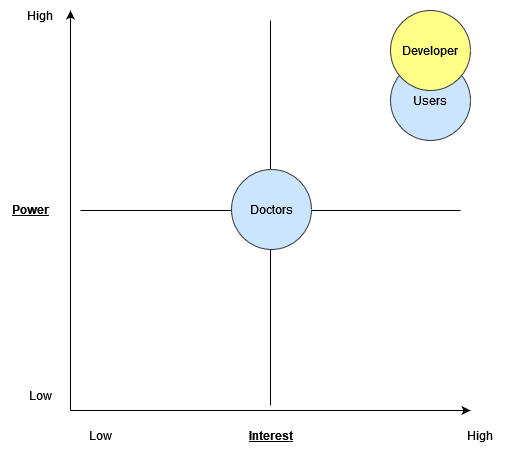
\includegraphics[scale=0.5]{stakeholder_diagram.png}
	\caption[Power/Interest Grid for Stakeholder-Analysis ]{Power/Interest Grid for Stakeholder-Analysis}
\end{figure}	

\section{System Context Diagram}
The greater environment in which a specific system or process functions is known as the system context. It covers all of the outside variables and influences that affect the system's function, such as the stakeholders who are impacted by its operation, the systems and processes with which it interacts, and the policies and regulations that it must comply with. The system context can be determined using the previously performed stakeholder analysis. Determining the system context helps to get an understanding of which components interact with the system. This includes both the stakeholders (groups) and systems that influence the system. The stakeholder groups of users and doctors can access the application via a smartphone. The developer communicates with the system via direct code-based access. The database, which is integrated externally, also communicates with the system via a code-based interface. There surely are some aspects about privacy policy and the security of personal data of the users. In the process of this work, the subject of legal issues with personal data is not addressed. 

\begin{figure}[h!]
	\centering
	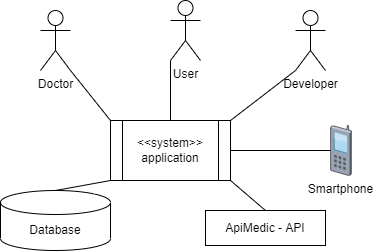
\includegraphics[scale=0.5]{system_context.png}
	\caption[System Context Diagram ]{System Context Diagram}
\end{figure}


\section{Requirements}
The requirements for an application can be divided into three categories: functional requirements, non-functional requirements and optional requirements. In this section, the different types of requirements are considered and created project-specifically.

\subsection{Functional Requirements}
Functional requirements are the specific capabilities, behaviors, and features that a system must have in order to fulfill its intended purpose. They describe what the system must do in order to be considered successful, and provide a basis for evaluating the system's performance and functionality. Functional requirements describe the functionality that an application should fulfil, i. e. the expected behavior of the system is captured by the functional requirements. The functional requirements of this system are shown in the appendix x.x. 
\begin{table}[H]
	\begin{center}
		\scriptsize
		\def\arraystretch{2}%
		\begin{tabularx}{\textwidth}{ c|c|c}
			\hline
			ID & Description & Figure \\
			\hline
			FR1 & The application must allow the user to switch between the tip and the diagnostics view & Abbildung \\
			\hline
			FR2 & The application must offer the user the option of being able to verify themselves as a doctor & Abbildung \\
			\hline
			FR3 & The application must offer a doctor the opportunity to log in & Abbildung \\
			\hline
			FR4 & The application must offer a doctor the opportunity to add a new record in the database & Abbildung \\
			\hline
			FR5 & The application must offer a doctor the possibility of editing data records in the database & Abbildung \\
			\hline
			FR6 & The application must allow a user to start a new diagnosis & Abbildung \\
			\hline
			FR7 & The application must enable a user to save a diagnosis & Abbildung \\
			\hline	
			FR8 &The application must enable a user to view his saved diagnoses again & Abbildung \\
			\hline
			FR10 &The application must allow a user to abort his diagnostic procedure at any time & Abbildung \\
			\hline
			FR11 & The application must allow a doctor to view his added records & Abbildung \\
			\hline
			FR12 & The application must allow a user to delete saved diagnoses & Abbildung \\
			\hline
			FR13 & The application must allow a user to view tips and tricks for symptoms and diseases & Abbildung \\
			\hline
			FR14 & The application must allow a doctor to abort adding/editing data & Abbildung\\
			\hline
		\end{tabularx}
		\normalsize
	\end{center}
	\caption{Functional Requirements}
\end{table}


\subsection{Non-functional Requirements}
After the functional requirements have been determined, the non-functional requirements are now considered. Non-functional requirements can be described by not dealing with the direct interaction of a user with the application, but with the system-specific properties. This includes, for example, the reliability of the application, but also safety aspects. [Buch google]

\begin{table}[H]
	\begin{center}
		\scriptsize
		\def\arraystretch{2}%
		\begin{tabularx}{\textwidth}{ c|c|c }
			\hline
			ID & Description & Figure \\
			\hline
			NFR1 & The application must make correct diagnoses & Abbildung \\
			\hline
			NFR1 & The application must make correct diagnoses & Abbildung \\
			\hline
			NFR2 & The application must be usable for patients without registration & Abbildung \\
			\hline
			NFR3 & The application must be usable for the user groups described & Abbildung \\
			\hline
			NFR4 & The application should have a graphical interface that can be used intuitively e & Abbildung \\
			\hline	
		\end{tabularx}
		\normalsize
	\end{center}
	\caption{Non-Functional Requirements}
\end{table}



\subsection{Optional Requirements}
As the name suggests, optional requirements of an application consist of requirements that do not necessarily have to be implemented. Their implementation is just a kind of bonus for the user.
\begin{table}[H]
	\begin{center}
		\scriptsize
		\def\arraystretch{2}%
		\begin{tabularx}{\textwidth}{ c|c|c }
			\hline
			ID & Description & Figure \\
			\hline
			OR1 & The application should make it possible to save and download a diagnosis in PDF format & Abbildung \\
			\hline
			OR2 & The application should make it possible for a user to save tips on a favorites list & Abbildung \\
			\hline	
		\end{tabularx}
		\normalsize
	\end{center}
	\caption{Optional Requirements}
\end{table}


\section{Use Cases}
The architectural goal of the application is to be designed to provide an optimal user experience for both, patients and doctors. In order to ensure this, it is necessary to determine before the actual development which use cases the software has to cover, i.e. the externally visible interactions of the users with the system. This ensures that the application meets the wishes of the users and that they actually use the application. In addition, possible ambiguities are revealed and required data structures are determined. Possible problems that may arise during use of the application are most likely to be found during the process and technical solutions can then be worked out. Experience has shown that use cases also make it easier for a developer to create the objects that have to be created with an object-oriented programming language in the early development process more precisely and to recognize and implement inheritance options at an early stage. Based on the functional requirements acquired from Chapter 3, use cases can now be created. Figure 3.3 shows the resulting use case diagram. 

\begin{figure}[h]
	\centering
	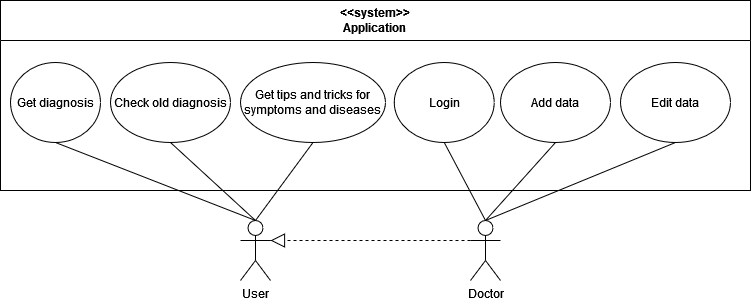
\includegraphics[scale=0.4]{use_case_diagram.png}
	\caption[Use Case Diagram]{Use Case Diagram}
\end{figure}

\subsection{Get Diagnosis}
\begin{table}[H]
	\begin{center}\scriptsize
		\def\arraystretch{2}%
		\begin{tabular}{ |c|c| } 
			\hline
			Name & Get Diagnosis \textbf{[FR6]}\\
			\hline	
			Description & The user wants to get a diagnosis, based on their symptoms \\ 
			\hline
			Result & The user receives a diagnosis \\ 
			\hline
			Actors & User, Doctor \\ 
			\hline
			Trigger & The user clicks on the new diagnosis button \\ 
			\hline
			Preconditions & None \\ 
			\hline
			Steps & \parbox{9cm}{\vspace{.5\baselineskip}
				1. The user clicks on the new diagnosis button\\
				2. The user selects his symptoms and specifies them\\
				3. The user indicates possible causes for his symptoms\\
				4. Diagnosis: the system determines possible diseases and presents them to the user and the use case ends}\\
			\hline
			Alternate flow & \parbox{9cm}{
				AF1a. The user wants to cancel the diagnosis and presses the stop button \textbf{[FR10]}\\
				AF1b. The system returns to the diagnostics view\\\\
				AF2a. The user wants to save the diagnosis \textbf{[FR7]}\\
				AF2b. The user presses the save button\\
				Af2c. The system saves the diagnosis}\\ 
			\hline
		\end{tabular}\normalsize
	\end{center}
	\caption{Use case get diagnosis}
\end{table}


\subsection{Review Received Diagnoses}
\begin{table}[H]
	\begin{center}\scriptsize
		\def\arraystretch{2}%
		\begin{tabular}{ |c|c| } 
			\hline
			Name & Review received diagnosis \textbf{[FR8]}\\
			\hline	
			Description & The user wants to review a diagnosis one more time \\ 
			\hline
			Result & The system shows the selected diagnosis to the user\\ 
			\hline
			Actors & User, Doctor \\ 
			\hline
			Trigger & Click on the diagnosis \\ 
			\hline
			Preconditions & The user has previously saved the diagnosis \\ 
			\hline
			Steps & \parbox{9cm}{\vspace{.5\baselineskip}1. The user selects the diagnosis from a list of previously stored diagnoses\\2. The system shows the selected diagnosis to the user \\ 3. When finished the user clicks on the back button}\\
			\hline
			Alternate flow & \parbox{9cm}{\vspace{.5\baselineskip}
				AF1a. The user wants to delete the diagnosis \textbf{[FR12]}\\
				AF1b. The user clicks on the delete button\\
				AF1c. The system deletes the diagnosis\\\\
				AF2a. The user wants to download the diagnosis as PDF\\
				AF2b. The user presses the download button}\\
			\hline
		\end{tabular}\normalsize
	\end{center}
	\caption{Use case review received diagnoses}
\end{table}

\subsection{Get Tips and Tricks for Symptoms and Diseases}
\begin{table}[H]
	\begin{center}\scriptsize
		\def\arraystretch{2}%
		\begin{tabular}{ |c|c| } 
			\hline
			Name & Get Tips and Tricks for Symptoms and Diseases \textbf{[FR13]}\\
			\hline	
			Description & The user wants to see tips and tricks regarading their symptoms \\ 
			\hline
			Result & The system shows the tip-view to the user\\ 
			\hline
			Actors & User, Doctor \\ 
			\hline
			Trigger & Click on the tip tab\\ 
			\hline
			Preconditions & None \\ 
			\hline
			Steps & \parbox{9cm}{\vspace{.5\baselineskip}
				1. The user selects the tip tab on the bottom navigation bar\\
				2. The system displays the tip-dashboard\\
				3. The user clicks on a tip to see the whole tip-description\\
				4. The system displays the tip-detail-page and the use case ends}\\
			\hline
			Alternate flow & \parbox{9cm}{\vspace{.5\baselineskip} 
				AF1a. The user wants to add a tip to his favorites \textbf{[OR2]}\\
				AF1b. The user clicks on the favorite icon of the tip\\
				AF1c. The system saves the tip to the users favorites }\\
			\hline
		\end{tabular}\normalsize
	\end{center}
	\caption{Use case get tups and tricks for sympstoms and diseases}
\end{table}



\subsection{Login}
\begin{table}[H]
	\begin{center}\scriptsize
		\begin{tabular}{ |c|c| } 
			\hline	
			Name & Login \textbf{[FR3]}\\ 
			\hline	
			Description & The user, a doctor, wants to log into the application \\ 
			\hline
			Goal & The doctor successfully logged into the system \\ 
			\hline
			Actors & Doctor \\ 
			\hline
			Trigger & Click on the login button \\ 
			\hline
			Preconditions & User is verified as a doctor \textbf{[FR3]} \\ 
			\hline
			Steps & \parbox{9cm}{\vspace{.5\baselineskip}
				1. The doctor clicks on the login button\\
				2. The systems shows the login form\\
				3. The doctor enters his personal details and presses the okay button\\
				4. The system checks for the credentials in the database\\
				5. The system displays the Add screen and the use case ends\\}\\
			\hline
			Alternate flow & \parbox{9cm}{\vspace{.5\baselineskip}
				AF1a. The system could not find the given credentials in the database\\
				AF1b. The user entered wrong credentials\\
				AF1c. The system displays an error message\\
				AF1d. The user retries\\\\
				AF2a. The user is not verfied as doctor yet \textbf{[FR3]}\\
				AF2b. The doctor enters his personal details and presses the okay button\\
				AF2c. The system starts the verification method\\
				AF2d. The doctor is verified as doctor\\
				AF2e. The system displays the Add screen and the use case ends\\}\\ 
			\hline
			Alternate flow (failure) & \parbox{9cm}{\vspace{.5\baselineskip}
				AFF1a. The user is no doctor\\
				AFF1b. The user is not able to verify himself as doctor\\
				AFF1c. The system shows an error}\\
			\hline
		\end{tabular}
	\end{center}\normalsize
	\caption{Use case login}
\end{table}


\subsection{Add Data}
\begin{table}[H]
	\begin{center}\scriptsize
		\begin{tabular}{ |c|c| } 
			\hline	
			Name & Add data to the databas  \textbf{[FR4]} \\
			\hline
			Description & The actor wants to add new data to the database \\ 
			\hline
			Goal & The data is added to the database \\ 
			\hline
			Actors & Doctor, Developer \\ 
			\hline
			Trigger & Click on the addData button \\ 
			\hline
			Preconditions & Actor is logged in \\ 
			\hline
			Steps & \parbox{9cm}{\vspace{.5\baselineskip}
				1. The actor clicks on the addData button\\
				2. The system shows the add form\\
				3. The actor enters the required data and presses the ok button\\
				4. The system adds the disease, symptom, cause or tip to the database\\ } \\
			\hline
			Alternate flow & \parbox{9cm}{\vspace{.5\baselineskip}
				AF1a. The actor missed to enter data\\
				AF1b. The system displays an error message\\
				AF1c. The actor retries\\\\
				AF2a. The actor wants to cancel the process \textbf{[FR12]}\\
				AF2b. The actor clicks on the cancel button\\
				AF2c. The system closes the add form}\\ 
			\hline
		\end{tabular}
	\end{center}\normalsize
	\caption{Use case add data}
\end{table}

\subsection{Edit Data}
\begin{table}[H]
	\begin{center}\scriptsize
		\begin{tabular}{ |c|c| }
			\hline
			Name & Edit Data \textbf{[FR5]} \\ 
			\hline	
			Description & The actor wants to edit old data \\ 
			\hline
			Goal & The edited data is uploaded to the database \\ 
			\hline
			Actors & Doctor, Developer \\ 
			\hline
			Trigger & Click on the edit button \\ 
			\hline
			Preconditions & Actor is logged in \\ 
			\hline
			Steps & \parbox{9cm}{\vspace{.5\baselineskip}
				1. The actor clicks on the edit button on the data he wants to edit\\
				2. The system shows the edit form\\
				3. The actor edits the data and presses the okay button\\
				4. The system updates the data and the use case ends
			}\\
			\hline
			Alternate flow & \parbox{9cm}{\vspace{.5\baselineskip}
				AF1a. The actor wants to cancel the process \textbf{[FR12]}\\
				AF1b. The actor clicks on the cancel button\\
				AF1c. The system closes the edit form}\\ \\ 
			\hline
		\end{tabular}
	\end{center}\normalsize
	\caption{Use case edit data}
\end{table}


\section{Domain Model}
Domain modeling is a major modeling topic in Agile development at scale because there is frequently a gap between comprehending the issue domain and the interpretation of requirements. It depicts the solution as a collection of domain objects that collaborate to satisfy system-level scenarios. [internetseite SAFe] The quintessence of the object-oriented analysis step is the decomposition of a domain into problem-relevant concepts or objects. A domain model is a visual representation of the problem-relevant domain classes of a domain. With the help of UML notation, a domain model is represented by a set of class diagrams in which no operations are defined, it presents a conceptual perspective and can show domain objects or classes, as well as associations between domain classes and attributes of domain classes. [UML 2 Buch]  Domain modeling is a major modeling topic in Agile development at scale because there is frequently a gap between comprehending the issue domain and the interpretation of requirements. Identifying domain entities and their connections, derived from a grasp of system-level requirements, offers a good foundation for understanding and supports practitioners in designing systems for maintainability, testability, and incremental development. [internetseite SAFe] Finding conceptual classes by recognizing substantive phrases is an effective technique to domain modeling. [Buch UML2] A potential course of action with the system is now built.

Actions
\begin{itemize}
	\item A person is a \textbf{user} of the application.
	\item A \textbf{user} chooses a \textbf{symptom} and specifies it.
	\begin{itemize}
		\item A \textbf{symptom} occurs in different \textbf{parts of the body}, has different \textbf{causes}, belongs to different \textbf{diseases} and has an average \textbf{duration}.
		\item A \textbf{user} specifies the selected symptom by narrowing down (selecting) \textbf{body parts}, \textbf{causes} and \textbf{time of appearance}.
	\end{itemize}
	\item One or more \textbf{user-specified symptoms} lead to the calculation of one or more \textbf{diseases}.
	\begin{itemize}
		\item A \textbf{disease} occurs in different \textbf{parts of the body}, has different \textbf{causes}, belongs to different \textbf{diseases} and has an average \textbf{duration}.
	\end{itemize}
	\item A \textbf{diagnosis} consists of one or more diseases.
	\item \textbf{Doctors} are special \textbf{users} of the application.
	\item \textbf{Doctors} can edit \textbf{tips}, \textbf{symptoms}, \textbf{causes} and \textbf{diseases}.
	\item \textbf{Doctors} can add \textbf{tips}, \textbf{symptoms}, \textbf{causes} and \textbf{diseases}.
	\item \textbf{Users} can view \textbf{tips}.  
\end{itemize}

The information just obtained makes it easier to create the domain model. The entities user, symptom, user-specified symptom, body part, diseases, causes, doctor, tip and diagnosis can already be recognized.
\begin{figure}[h]
	\centering
	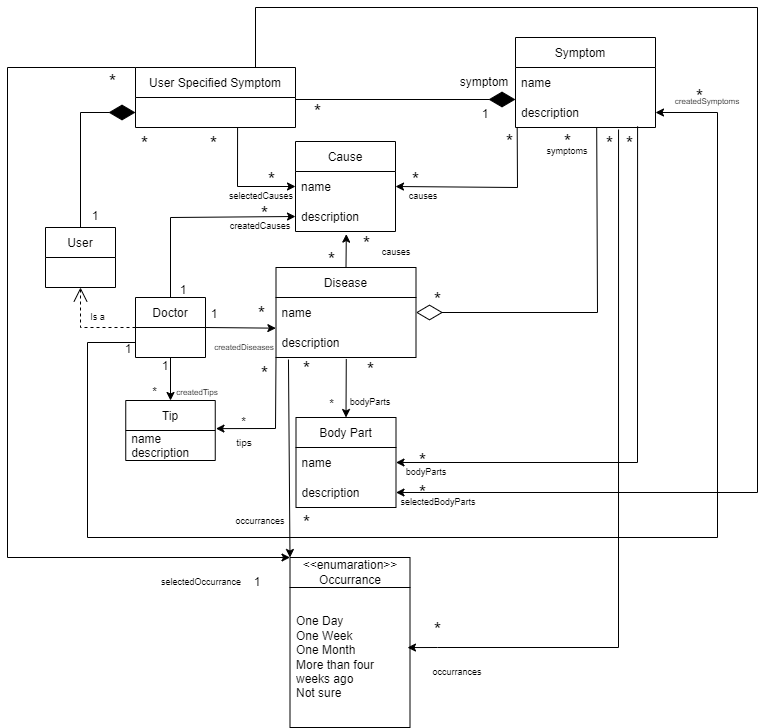
\includegraphics[scale=0.65]{domain_model.png}
	\caption[Domain Model]{Domain Model}
\end{figure}


